\documentclass[11pt,a4paper]{ivoa}

\usepackage{xcolor}  % for colored text
\usepackage{longtable}
\usepackage{array}
\usepackage{colortbl}

\usepackage{listings}
\lstset{ %
  backgroundcolor=\color{white},   % choose the background color; you must add \usepackage{color} or \usepackage{xcolor}
  basicstyle=\scriptsize\ttfamily,        % the size of the fonts that are used for the code
  breakatwhitespace=false,         % sets if automatic breaks should only happen at whitespace
  breaklines=true,                 % sets automatic line breaking
  captionpos=b,                    % sets the caption-position to bottom
  frame=single,                    % adds a frame around the code
  keepspaces=true,                 % keeps spaces in text, useful for keeping indentation of code (possibly needs columns=flexible)
  language={},                 % the language of the code
  otherkeywords={*,...},            % if you want to add more keywords to the set
  numbers=none,                    % where to put the line-numbers; possible values are (none, left, right)
  rulecolor=\color{black},         % if not set, the frame-color may be changed on line-breaks within not-black text (e.g.comments (green here))
  showspaces=false,                % show spaces everywhere adding particular underscores; it overrides 'showstringspaces'
  showstringspaces=false,          % underline spaces within strings only
  showtabs=false,                  % show tabs within strings adding particular underscores
  tabsize=2,                       % sets default tabsize to 2 spaces
  title=\lstname                   % show the filename of files included with \lstinputlisting; also try caption instead of title
}

\input tthdefs
\input gitmeta

\title{HATS: A Standard for the Hierarchical Adaptive Tiling Scheme in the Virtual Observatory}

% Borrowed from UCDList.tex
% having descriptions in a narrow column is painful -- the following
% is an attempt to define a suitable column style ("D"escription)
\newcolumntype{D}[1]{>{\raggedright\tolerance=7000\let\newline\\\arraybackslash
  \hspace{0pt}}p{#1}}

\ivoagroup{Applications Group}

\author[https://www.ivoa.net/authors/caplar]{Neven Caplar}
\author[https://www.ivoa.net/authors/delucchi]{Melissa DeLucchi}
\author[https://www.ivoa.net/authors/beebe]{Wilson Beebe}
\author[https://www.ivoa.net/authors/branton]{Doug Branton}
\author[https://www.ivoa.net/authors/campos]{Sandro Campos}
\author[https://www.ivoa.net/authors/jones]{Derek Jones}
\author[https://www.ivoa.net/authors/malanchev]{Konstantin Malanchev}
\author[https://www.ivoa.net/authors/mcguire]{Sean McGuire}
\author[https://www.ivoa.net/authors/lynn]{Olivia Lynn}
\author[https://www.ivoa.net/authors/juric]{Mario Juric}

\editor{editor here}

\previousversion{This is the first public release}

\begin{document}
\textcolor{red}{KOSTYA NOTE - Should we add people from the HATS working group? Those who contributed code to HATS/LSDB?}
\begin{abstract}
The increasing complexity and volume of astronomical datasets necessitate efficient spatial indexing and query strategies within the Virtual Observatory (VO). 
The Hierarchical Adaptive Tiling Scheme (HATS) is a framework designed to facilitate scalable queries, filtering operations, and efficient data retrieval across large astronomical surveys. 
Traditional spatial indexing methods often struggle with the massive scale of modern astronomical datasets, leading to inefficient query execution and storage overhead. 
HATS provides a flexible, hierarchical approach that balances computational efficiency and adaptability to non-uniform data distributions.\par

This document describes the structure, implementation, and best practices for integrating HATS within the VO ecosystem, ensuring interoperability and performance optimization for distributed astronomical datasets. We discuss how HATS enhances existing indexing schemes, its role in federated data access, and how it enables powerful applications for large-scale survey science and efficient cross-matching of astronomical catalogs. \par 
The reference implementation of HATS can be found at \url{https://github.com/astronomy-commons/hats}. 
\textcolor{red}{KOSTYA NOTE - We don't give a use-case, for example, we can say that it is to enable fast querying of >~1e6 rows}

\end{abstract}

\section*{Acknowledgments}
The authors thank the IVOA Applications Working Group and various contributors from the astronomical community for their feedback and discussions that shaped this standard. 
We acknowledge the key collaborations with the Space Telescope Science Institute (STScI) and IPAC, at Caltech, whose expertise and contributions have been invaluable in refining the HATS framework. 
Additionally, we extend our gratitude to  the Strasbourg astronomical Data Center (CDS) for their assistance in metadata structuring and interoperability support. 
This work has also benefited from insights provided by the S-Plus survey, Linea, European Space Agency, and Canadian Astronomy Data Center (CADC), whose contributions have helped enhance the applicability and robustness of HATS in large-scale astronomical data analysis. \par

This project is supported by Schmidt Sciences.
This project is based upon work supported by the National Science Foundation under Grant No. AST-2003196.
This project acknowledges support from the DIRAC Institute in the Department of Astronomy at the University of Washington. The DIRAC Institute is supported through generous gifts from the Charles and Lisa Simonyi Fund for Arts and Sciences, and the Washington Research Foundation.


\section*{Conformance-related definitions}
The words ``MUST'', ``SHALL'', ``SHOULD'', ``MAY'', ``RECOMMENDED'', and
``OPTIONAL'' (in upper or lower case) used in this document are to be
interpreted as described in IETF standard RFC2119 \citep{std:RFC2119}.

The \emph{Virtual Observatory (VO)} is a
general term for a collection of federated resources that can be used
to conduct astronomical research, education, and outreach.
The \href{https://www.ivoa.net}{International
Virtual Observatory Alliance (IVOA)} is a global
collaboration of separately funded projects to develop standards and
infrastructure that enable VO applications.

\section{Introduction}
The rapid expansion of astronomical data from large survey facilities like Vera C. Rubin Observatory, Euclid, and Roman Space Telescope necessitates innovative solutions for spatial indexing and efficient data retrieval. 
These surveys generate vast amounts of high-resolution imaging and time-domain data, requiring efficient methods for organizing, querying, and cross-matching data across multiple archives. 
Traditional approaches to spatial indexing, such as hierarchical pixelization (e.g., HEALPix) or static tiling schemes, often exhibit inefficiencies when handling uneven sky densities.
\textcolor{red}{KOSTYA NOTE - "dynamic" may be misunderstood, as the partitioning is not happening on-the-fly}

The Hierarchical Adaptive Tiling Scheme (HATS) is a novel approach designed to optimize spatial data partitioning while maintaining flexibility in accommodating varying data densities. 
Unlike fixed spatial partitioning methods, HATS adaptively adjusts tile sizes based on local data characteristics, ensuring an optimal balance between resolution, query efficiency, and storage management. 
By leveraging a hierarchical structure, HATS allows users to perform efficient spatial queries while preserving high precision in regions of interest.
\textcolor{red}{KOSTYA NOTE - Readers may not understand that "multi-resolution" is about healpix order}

This document aims to define best practices for implementing and utilizing this tiling scheme within the Virtual Observatory framework. 
This document outlines the principles behind HATS, describes its data model, and provides recommendations. 
Additionally, we discuss how HATS can facilitate efficient cross-matching of astronomical catalogs, accelerate large-scale spatial queries, and enhance interoperability between diverse astronomical datasets.

\section{Motivation and Goals}
The primary motivation behind HATS is to address the following challenges in astronomical data management:
\begin{itemize}
    \item \textbf{Scalability:} Modern astronomical surveys generate petabytes of spatially distributed data, requiring an indexing scheme that scales efficiently with dataset size.
    HATS provides such an indexing scheme, and creates files whose properties and size are well-suited to parallel operations.
    \item \textbf{Adaptive Spatial Resolution:} Fixed grid-based partitioning often leads to inefficient storage and query execution, particularly in non-uniformly distributed datasets. 
    HATS adaptively adjusts tile sizes to accommodate varying data densities.
    \item \textbf{Efficient Query Execution:} Spatial queries such as nearest-neighbor searches and cross-matching must be executed efficiently across distributed data repositories. 
    HATS enables rapid indexing and retrieval of relevant data subsets, and provides an balanced partitioning of data for distributed parallel processing.
    \item \textbf{Interoperability:} Astronomical data is collected from diverse instruments and observatories, often using different spatial reference frames. 
    HATS provides a standardized framework for integrating and harmonizing spatial data across multiple repositories.
\end{itemize}

\section{HATS Design and Implementation}

\subsection{HATS Catalog Directory Structure} \label{sec:catalog}

The HATS framework relies on spatially sharding catalogs into Parquet files of approximately the same size 
Here, we discuss how this is achieved and additional concepts that make it easier to use this main idea for astronomical research.

The central unit of data storage is the HATS \texttt{catalog}. 
It stores the data along with the associated metadata needed to access it. 
The  \texttt{catalog} organization structure is shown in Listing~\ref{fig:exampleCatalogStructure}.

\begin{minipage}{\linewidth}
\begin{lstlisting}[caption=Example catalog directory contents, label=fig:exampleCatalogStructure]
catalog/
|-- [REQUIRED] properties
|-- [RECOMMENDED] partition_info.csv
|-- [OPTIONAL] point_map.fits
|-- [OPTIONAL] data_thumbnail.parquet
+-- dataset/
    |-- [RECOMMENDED] _metadata
    |-- [RECOMMENDED] _common_metadata
    |-- Norder=0/
    |-- Norder=1/
    |-- Norder=2/
    |-- Norder=3/
    |-- Norder=4/
    |-- Norder=5/
    |-- Norder=6/
    +-- Norder=. . ./
\end{lstlisting}
\end{minipage}

The astronomy data is stored in the directory \texttt{dataset}, and further, within the subdirectories that specify the order at which particular part of the dataset is stored. 
We will discuss the partitioning and data storage in Sections~\ref{sec:hierarchical}, \ref{sec:adaptive} and \ref{sec:parquet}. 
The other files visible above are various metadata and auxiliary files that are here to enable better and easier handling of the data and we will describe them in Section~\ref{sec:meta}. 
    
\subsubsection{Hierarchical Directory Structure} \label{sec:hierarchical}
Focusing now on the dataset's contents, HATS employs a multi-level hierarchy based on HEALPix tiling.
Each level corresponds to a single HEALPix order and represents a progressively finer spatial resolution.

All tiles of the same HEALPix order are contained within the same prefix \texttt{Norder=k} directory. 
To avoid directories becoming too large for some file systems, the tiles are then grouped by a \texttt{Dir} subdirectory prefix,
where the value of the \texttt{Dir} key is the result of integer division by 10,000 of the pixel number.

We see the directory structure in Listing~\ref{fig:datasetWithLeaf}, showing a dataset with leaf parquet files at several HEALPix orders.

\begin{minipage}{\linewidth}
\begin{lstlisting}[caption=Example catalog dataset directory contents, label=fig:datasetWithLeaf]
dataset/
|-- . . .
|-- Norder=6/
|   |-- Dir=0/
|   |   |-- Npix=0.parquet
|   |   |-- . . .
|   |   +-- Npix=9999.parquet
|   +-- Dir=10000/
|       +-- Npix=10000.parquet
|           +-- . . .
|-- Norder=7/
+-- . . .
\end{lstlisting} 
\end{minipage}

The data is stored in the parquet files (discussed in Section \ref{sec:parquet}), with one or multiple files being possible in the final directory, i.e., in the ultimate data leaf.  \par 
If there are multiple files representing a single data partition, they should be read together, i.e., we consider them to be one single data unit. 
In this way, small updates can be added to already existing  \texttt{catalogs} with simple, correctly placed, additions of files in existing folders.

Such a directory structure would appear as shown in Listing~\ref{fig:datasetWithDir}.

\begin{minipage}{\linewidth}
\begin{lstlisting}[caption=Example catalog dataset directory contents with leaf directories, label=fig:datasetWithDir]
dataset/
|-- . . .
|-- Norder=6/
|   |-- Dir=0/
|   |   |-- Npix=0/
|   |   |   |-- part0.parquet
|   |   |   +-- . . .
|   |   +-- Npix=9999/
|   |       |-- part0.parquet
|   |       +-- . . .
|   +-- Dir=10000/
|       +-- Npix=10000/
|           |-- part0.parquet
|           +-- . . .
|-- Norder=7/
+-- . . .
\end{lstlisting} 
\end{minipage} 

\subsubsection{Adaptive Tiling Algorithm} \label{sec:adaptive}
Unlike static partitioning schemes, HATS adaptively subdivides spatial regions based on data angular density. 
In areas with sparse data, larger HEALPix tiles minimize storage overhead, whereas high-density areas are subdivided into smaller tiles to improve query efficiency. \par

The data is stored at a given level until the size of the data within the tile crosses a predetermined threshold. 
This threshold can be, most commonly, the number of rows or the size of the data on the disk. 
As we add the data, at the point that the threshold is reached, the data gets split into four higher-order HEALPix tiles using the spatial information contained in the data. 
This process continues until all of the data is stored at the appropriate level and no data leaf has more data than the predetermined threshold. We show an example of the result of this procedure in Figure \ref{fig:order}.

\begin{figure}
\centering
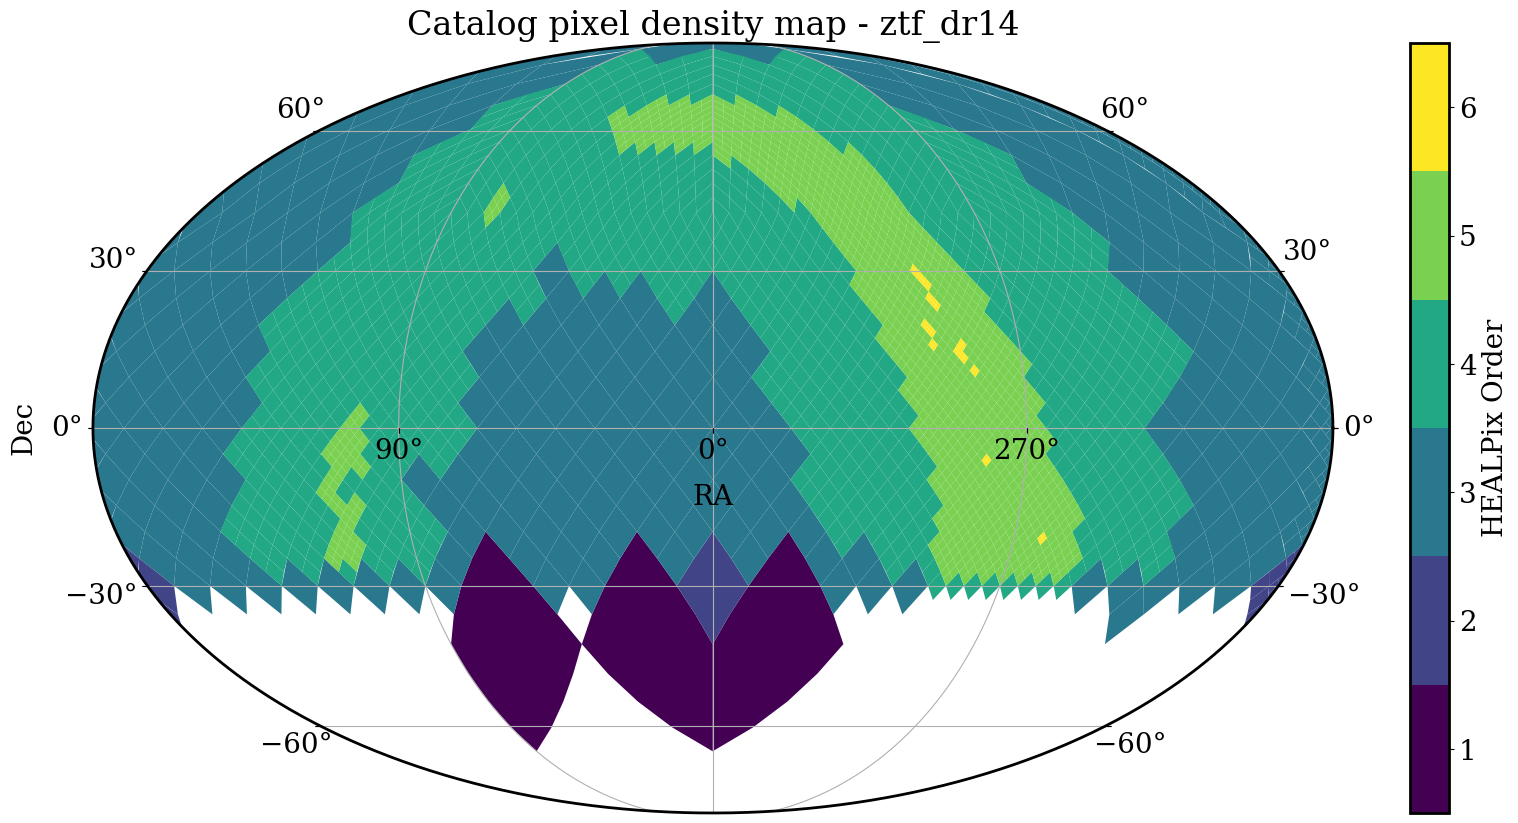
\includegraphics[width=0.9\textwidth]{order-pix.png}
\caption{Adaptive tiling for the object catalog of Zwicky Transient Facility, Data Release 14 \citep{ztf:Bellm2019, ztf:Masci2019} To achieve a similar number of rows across the entire sky, we partition the galactic region more finely. This results in tiles of higher HEALPix order in the galactic plane, particularly near the galactic bulge. }
\label{fig:order}
\end{figure}


\subsubsection{Structure of Data Files} \label{sec:parquet}
The astronomical data is stored in Parquet format \footnote{\href{https://parquet.apache.org}{https://parquet.apache.org}}.
Parquet is a binary columnar storage file format optimized for efficient data compression and retrieval, especially well-suited for analytical workloads. 
It is ideal for storing large amounts of astronomical tabular data because it allows fast access to specific columns without reading the entire dataset, significantly reducing I/O and improving performance. \par

The HATS format RECOMMENDS that the first column of the dataset is the \texttt{\_healpix\_29} index column.  
\texttt{\_healpix\_29} stores the crucial spatial information about the position in the sky for each row, and it is not unique.
This is calculated as the HEALPix order 29 value of the row's right ascension and declination. 
If two objects occur at the same location (or the data is individual observations of the same sky object), then multiple rows may have the same value for the \texttt{\_healpix\_29} column.
The existence of this value speeds up downstream spatial calculations, and is beneficial for spatially-intensive applications.

Additional optional performance considerations for Parquet files is discussed in Section~\ref{sec:parquetPerformance}.

\subsection{Supplemental Tables} \label{sec:supplemental}

To improve scalability and efficient query optimization, HATS readers can benefit from alternative arrangements of the data. 
We refer to these as supplemental tables or supplemental catalogs, and these offer a limited or re-projected view of the primary dataset.

\subsubsection{Margin Cache} \label{sec:margin}

One of the primary motivations for HATS is the rapid cross-matching of different surveys or different data sources within the same survey. 
The power of cross-matching in HATS is that each computation unit gets small spatially-connected parts from each dataset and works on them one part at a time,
with the amount of data being roughly equal in each part, for best efficiency.\par 

However, this introduces a limitation: at the boundaries of a divided section, some data points that should be cross-matched will be missed because they are present just across the border in neighboring partitions instead.
This has a number of causes (observational error, non-point source positions, proper motion, etc), but it should be handled by applications to ensure the appropriate counterpart is found during cross-matching.\par

One option would be to load all neighboring partitions when performing a cross-match. 
However, this would require loading much unnecessary data, as only a small sliver around the edge of a partition is a candidate for counterparts in neighboring partitions. 
Figure~\ref{fig:margin} shows some example data points that are near to a HEALPix tile boundary, and should be included in a cross-match calculation.

\begin{figure}
\centering
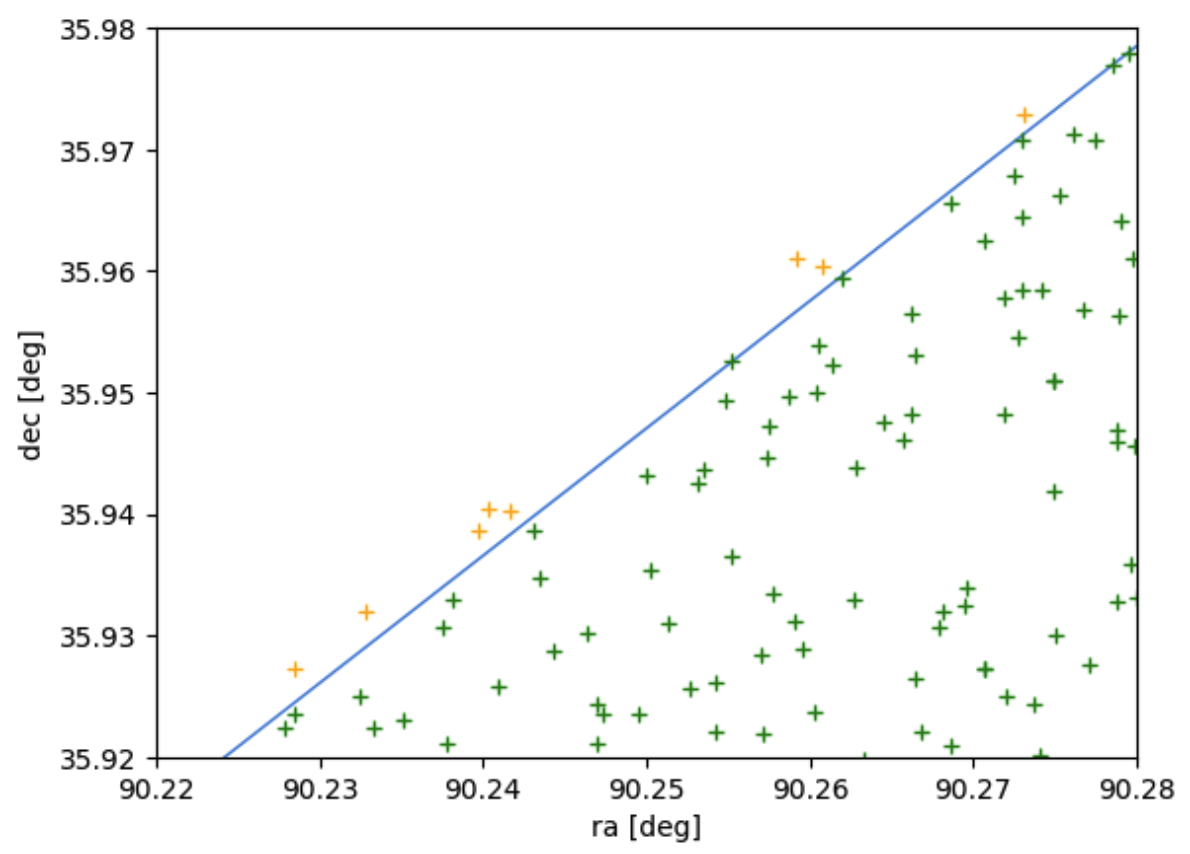
\includegraphics[width=0.9\textwidth]{margin-pix.png}
\caption{Example of margin contents. Green points are present in the primary catalog partition, the blue line is the HEALPix pixel boundary, and yellow points are points in the neighboring tile that are within 10 arcseconds of the boundary.}
\label{fig:margin}
\end{figure}

We address this through the creation of a margin cache.
This is an additional catalog that contains points in a limited angular threshold around the primary catalog partition.
The margin catalog MUST contain all points within the indicated angular threshold from the tile boundary, but MAY contain additional points, either for simplicity of spatial calculations, or to provide additional points of interest.\par

The margin data can be loaded alongside the primary catalog partition data during a cross-match operation to account for any positional issues that may arise around the boundaries of the partition's HEALPix pixel.
The margin catalog can be overloaded to also provide a cache of related objects that are not within the primary data partition for other scientific use cases.

\subsubsection{Index Table} \label{sec:index}
\textcolor{red}{KOSTYA NOTE - We never specify the coordinate system in the doc}
\textcolor{red}{MELISSA NOTE TO KOSTYA NOTE - YES - that seems like something we should discuss, since make a lot of assumptions about using the same coordinate system in all catalogs, for cross-matching purposes}
HATS catalogs are partitioned spatially, on right ascension and declination. 
This makes finding objects in a particular area of the sky very straightforward. 
However, one may occasionally only know the object by the survey-assigned identifier, and to find the row, would have to perform a full scan of all partitions. \par

HATS supports creating additional secondary index tables. 
To create index tables, we perform a full scan over all of the data, sort by the desired column, and write out a simple mapping from the unique identifier to where it can be found in the sky.
Sorting over such a large dataset can be expensive, and it's preferable to perform this operation once and store the results. \par

This mirrors the relational database notion of a lookup table, where you can lookup the spatial parameters of a non-spatial property.
The user can query the index catalog for the HEALPix tile where the value can be found, and then only need to load the primary catalog partition for the corresponding HEALPix tile. 
This greatly speeds up and facilitates the query, as we now only have to load a single tile instead of going through the whole catalog.
These are general secondary indexes, and can be built on any column, not just the survey-assigned identifier.

\subsubsection{Catalog Collection} \label{sec:collection}

Margins and indexes are associated with a single astronomical dataset, and to make this connection clearer and enable friendlier application behavior, tables MAY be grouped together under a single directory called a catalog collection.
These include the primary data \texttt{catalog} and other \texttt{catalogs} that are optional and are intended either to improve access to the main \texttt{catalog} or to enrich it with additional information. 

In Listing~\ref{fig:exampleCollectionStructure}, we present an overview of this folder structure, including a few common examples of such optional catalogs.
The catalog collection directory MUST contain a \texttt{collection.properties} file, whose content is outlined in Section~\ref{sec:collectionProperties}.

\begin{minipage}{\linewidth}
\begin{lstlisting}[caption=Example collection directory contents, label=fig:exampleCollectionStructure]
gaia_dr3/
|-- collection.properties
|-- catalog/
|   |-- properties
|   +-- . . .
|-- [OPTIONAL] margin_5arcs/
|   |-- properties
|   +-- . . .
|-- [OPTIONAL] margin_10arcs/
|   |-- properties
|   +-- . . .
+-- [OPTIONAL] index_designation/
    |-- properties
    +-- . . .
\end{lstlisting}
\end{minipage}

\subsubsection{Association Table} \label{sec:association}

Noting again that cross-matching and multi-survey analysis is a primary motivator for the HATS spatial format, we introduce the HATS association table. 

This table provides a spatially-sharded set of links between rows in two different object catalogs. 
This mirrors the relational database notion of a link table, and will likely be composed of the primary survey identifiers from either side of the association.
We make no prescription as to whether the relationships are one-to-one or one-to-many. \par

There is a single "primary" catalog that reflects the left side, and the other catalog is the "join" catalog (as the data can be joined into the primary catalog).
The resulting association data will use the coordinates of the primary catalog, and MAY be partitioned with the same pixels as the primary catalog.
If there are many more or many fewer association links than there are objects in the primary table, it may be preferable to either combine or split the leaf parquet files further.

% \subsubsection{Map Catalog} \label{sec:mapCatalog}
% \textcolor{red}{TODO: we should mention this, as it's very useful for science. }

\subsection{Metadata and Auxiliary Files} \label{sec:meta}
HATS implementations utilize auxiliary files and metadata files to store relevant information about the  structure, including:
\begin{itemize}
    \item \textbf{[REQUIRED] properties}, at  \texttt{catalog} level    
    \item \textbf{[RECOMMENDED] partition\_info.csv}, at  \texttt{catalog} level
    \item \textbf{[RECOMMENDED] partition\_join\_info.csv}, at  \texttt{catalog} level
    \item \textbf{[OPTIONAL] point\_map.fits}, at  \texttt{catalog} level
    \item \textbf{[OPTIONAL] data\_thumbnail.parquet}, at  \texttt{catalog} level
    \item \textbf{[RECOMMENDED] \_metadata}, at  \texttt{catalog/dataset} level
    \item \textbf{[RECOMMENDED] \_common\_metadata}, at  \texttt{catalog/dataset} level
    \item \textbf{[REQUIRED] collection.properties}, at  \texttt{catalog} collection level
\end{itemize}
    
Note that collection.properties is only required if creating a \texttt{catalog} collection for your dataset. \par 
We will now go over these files and explain their function, format and their contents. 
    
\subsubsection{properties} 

A text file named \texttt{properties} is REQUIRED in the root level of the catalog directory.
It marks the directory as containing a HATS catalog, and so MUST be located in the root directory of the catalog.
It MUST be encoded in UTF-8, with one line per property, following the syntax \texttt{keyword = value}.
The ordering of the keywords is not important. The keywords MAY include many of those listed in Table~\ref{tab:properties}.

The text file may contain comment lines, beginning with the \texttt{'\#'} character.

An example \texttt{properties} file is shown in Listing~\ref{fig:examplePropertiesFile}.

\begin{minipage}{\linewidth}
\begin{lstlisting}[caption=Example \texttt{properties} file contents, label=fig:examplePropertiesFile]
#HATS catalog
obs_collection=euclid_q1_merFinalCatalog
dataproduct_type=object
hats_nrows=29767806
hats_col_ra=RIGHT_ASCENSION
hats_col_dec=DECLINATION
hats_cols_sort=OBJECT_ID
hats_max_rows=1000000
hats_order=6
moc_sky_fraction=0.00618
hats_builder=hats-import v0.4.4
hats_creation_date=2025-03-20T03\:38UTC
hats_estsize=23137775
hats_release_date=2024-09-18
hats_version=v0.1
\end{lstlisting}
\end{minipage}

We enforce additional requirements for the presence of particular fields for different types of HATS tables. 
A matrix of these requirements is shown in Table~\ref{tab:propertyRequirements}.

{\footnotesize
\begin{longtable}[h!]{D{0.33\textwidth} D{0.67\textwidth}}
\sptablerule
\textbf{HATS Keyword}&\textbf{Description - Format - Example}\\
\sptablerule
\endhead

addendum\_did &If content has been added after initial catalog creation, creator\_did of any added data \\
all\_indexes &For catalog collections, space-delimited map of indexed field to subdirectories containing index tables. \\
all\_margins &For catalog collections, space-delimited list of subdirectories containing margin caches. \\
bib\_reference &Bibliographic reference \\
bib\_reference\_url &URL to bibliographic reference \\
creator\_did &Unique ID of the HATS - Format: IVOID - Ex : ivo://CDS/P/2MASS/J \\
data\_ucd &UCD describing data contents \\
dataproduct\_type &Format: one word ONE OF(object, margin, association, index, ...) \\
default\_index &For catalog collections, the field of the default index to use for ID searches. \\
default\_margin &For catalog collections, the subdirectory containing the default margin cache to use for cross-matching \\
hats\_assn\_join\_table\_url &For association tables, there will be a join table with original survey data (right side of the join) \\
hats\_assn\_leaf\_files &For association tables, does the table contain leaf files (may optionally only provide a "soft" association between tiles only). \\
hats\_builder &Name and version of the tool used for building the HATS. Format: free text -- Example "hats-import v0.6.4" \\
hats\_col\_assn\_join &For association tables,column name for the joining (right) side of the join within the original table \\
hats\_col\_assn\_join\_assn &For association tables, column name in the assocation table for the join (right) side of the association table. \\
hats\_col\_assn\_primary &For association tables, column name for the primary (left) side of the join \\
hats\_col\_assn\_primary\_assn &For association tables, column name in the association table that matches the primary (left) side of the join \\
hats\_col\_dec &Column name of the dec coordinate. Used for partitioning and default cross-matching. \\
hats\_col\_ra &Column name of the ra coordinate. Used for partitioning and default cross-matching. \\
hats\_cols\_default &Which columns should be read from parquet files, when user doesn't otherwise specify. Useful for wide tables. Format: space-delimited column names \\
hats\_cols\_sort &At catalog creation time, the columns used to sort the data, in addition to \texttt{\_healpix\_29} column. \\
hats\_cols\_survey\_id &The primary key used in the original survey data. May be multiple columns if the survey uses a composite key (e.g. object ID and MJD for detections) \\
hats\_coordinate\_epoch &For the default ra and dec (hats\_col\_ra, hats\_col\_dec), the measurement epoch \\
hats\_copyright &Copyright mention associated to the HATS - Format: free text \\
hats\_creation\_date &HATS first creation date - Format: ISO 8601 => YYYY-mm-ddTHH:MMZ \\
hats\_creator &Institute or person who built the HATS. Format: free text. Ex : CDS (T.Boch) \\
hats\_estsize &HATS size estimation. Format: positive integer. Unit : KB \\
hats\_frame &Coordinate frame reference. Format: word "equatorial" (ICRS), "galactic", "ecliptic" \\
hats\_index\_column &For index tables, the column that is indexed over \\
hats\_index\_extra\_column &For index tables, extra columns that are carried through with the index \\
hats\_margin\_threshold &For margin tables, the threshold used for finding points within margin. Units: arcs \\
hats\_max\_rows &At catalog creation time, the maximum number of rows per file before breaking into 4 new files at higher order. \\
hats\_nrows &Number of rows of the HATS catalog. Format: positive integer \\
hats\_order &Deepest HATS order. Format: positive integer \\
hats\_primary\_table\_url &For supplemental tables, there will be a primary table with original survey data. Format: URL\\
hats\_progenitor\_url &URL to an associated progenitor HATS catalog. Format: URL \\
hats\_release\_date &Last HATS update date - Format: ISO 8601 => YYYY-mm-ddTHH:MMZ \\
hats\_service\_url &HATS access url. Format: URL \\
hats\_status &HATS status. Format: list of space-delimited words ("private" or "public"), ("main", "mirror", or "partial"), ("clonable", "unclonable" or "clonableOnce"). Default : public main clonableOnce \\
hats\_version &Number of HATS version. Format: 0.1 (corresponds to version of this note) \\
moc\_sky\_fraction &Fraction of the sky covered by the MOC associated to the HATS. Format: real between 0 and 1 \\
npix\_suffix & String to indicate file suffix for leaf files. In the typical HATS directory structure, this is \texttt{'.parquet'} or \texttt{'.pq'} because there is a single file in each Npix partition. If using leaf directories, \texttt{'/'}. \\
obs\_ack &Acknowledgment mention. \\
obs\_collection &Short name of original data set. Format: one word. Ex : 2MASS \\
obs\_copyright &Copyright mention associated to the original data. Format: free text \\
obs\_copyright\_url &URL to a copyright mention \\
obs\_description &Data set description. Format: free text, longer free text description of the dataset \\
obs\_regime &General wavelength. Format: word: "Radio" | "Millimeter" | "Infrared" | "Optical" | "UV" | "EUV" | "X-ray" | "Gamma-ray" \\
obs\_title &Data set title. Format: free text, one line. Ex : HST F110W observations \\
prov\_progenitor &Provenance of the original data. Format: free text \\
publisher\_id &Unique ID of the HATS publisher. Format: IVOID - Ex : ivo://CDS \\
t\_max &Stop time of the observations. Format: real. Representation: MJD \\
t\_min &Start time of the observations. Format: real. Representation: MJD \\
\sptablerule    
\caption{Available keys for properties file}
\label{tab:properties}
\end{longtable}}

\begin{table}[h!]
\rowcolors{2}{white}{gray!20}
{\footnotesize\begin{tabular}{l c c c c c}
\sptablerule
\textbf{HATS Keyword} &\multicolumn{5}{c}{\textbf{HATS Catalog Type}} \\
\rowcolor{white}
& object & margin & index & association  & collection \\
\sptablerule
all\_indexes & & & & &opt \\
all\_margins & & & & &opt \\
dataproduct\_type &REQ &REQ &REQ &REQ & \\
default\_index & & & & &opt \\
default\_margin & & & & &opt \\
hats\_assn\_join\_table\_url & & & &REQ & \\
hats\_assn\_leaf\_files & & & &REQ & \\
hats\_col\_assn\_join & & & &REQ & \\
hats\_col\_assn\_join\_assn & & & &opt & \\
hats\_col\_assn\_primary & & & &REQ & \\
hats\_col\_assn\_primary\_assn & & & &opt & \\
hats\_col\_dec &REQ &opt & & & \\
hats\_col\_ra &REQ &opt & & & \\
hats\_cols\_default &opt &opt & & & \\
hats\_index\_column & & &REQ & & \\
hats\_index\_extra\_column & & &opt & & \\
hats\_margin\_threshold & &REQ & & & \\
hats\_npix\_suffix &opt &opt &opt &opt & \\
hats\_nrows &REQ &REQ &REQ &REQ & \\
hats\_primary\_table\_url & &REQ &REQ &REQ &REQ \\
obs\_collection &REQ &REQ &REQ &REQ &REQ \\
\sptablerule
\end{tabular}}
\caption{Catalog-type specific fields. For display, REQ is REQUIRED, and opt is OPTIONAL}
\label{tab:propertyRequirements}
\end{table}

\subsubsection{partition\_info.csv} 

A text file named \texttt{partition\_info.csv} is OPTIONAL and RECOMMENDED in the root level of the catalog directory.
If present, it MUST be a CSV (comma-separated-values) file, with the columns \texttt{"Norder"} and \texttt{"Npix"}, as shown in example contents in Listing~\ref{fig:examplePartitionInfoCsv}.
Additional columns might be present in the file, but are not required, and may not be interpreted by all HATS readers.
The values of pairs of \texttt{"Norder"} and \texttt{"Npix"} reflect the HEALPix tiles of the catalog's partitions. 
HATS readers can quickly read this file to understand the full scope of the catalog, and potential spatial overlap with other catalogs.

\begin{minipage}{\linewidth}
\begin{lstlisting}[caption=Example \texttt{partition\_info.csv} file contents, label=fig:examplePartitionInfoCsv]    
Norder,Npix
3,530
4,637
4,958
4,1003
4,2147
\end{lstlisting}
\end{minipage}

\subsubsection{partition\_join\_info.csv} 

A text file named \texttt{partition\_join\_info.csv} is OPTIONAL and RECOMMENDED in the root level of the catalog directory for an association catalog.
If present, it MUST be a CSV (comma-separated-values) file, with the columns \texttt{"Norder"}, \texttt{"Npix"}, \texttt{"join\_Norder"}, and \texttt{"join\_Npix"}, as shown in example contents in Listing~\ref{fig:examplePartitionJoinInfoCsv}.
Additional columns might be present in the file, but are not required, and may not be interpreted by all HATS readers.
The values of pairs of \texttt{"Norder"} and \texttt{"Npix"} reflect the HEALPix tiles of the primary catalog's partitions. 
The corresponding values of pairs of \texttt{"join\_Norder"} and \texttt{"join\_Npix"} reflect the HEALPix tiles of the join catalog's partitions that have matches inside the primary catalog's partition.
HATS readers can quickly read this file to understand the full spatial overlap with other catalogs, and plan which leaf partitions of the primary and join catalogs will be loaded. \par

This file is not used for table types that are NOT association tables.

\begin{minipage}{\linewidth}
\begin{lstlisting}[caption=Example \texttt{partition\_join\_info.csv} file contents, label=fig:examplePartitionJoinInfoCsv]    
Norder,Npix,join_Norder,join_Npix
3,530,3,517
3,530,4,2120
3,530,4,2121
3,530,4,2122
4,637,4,637
\end{lstlisting}
\end{minipage}

\subsubsection{point\_map.fits} 

A FITS file containing the MOC (multi-order coverage map) of the catalog.
This is a two-dimensional histogram of points in each HEALPix tile at some reasonably high order.
This will be at the highest order calculated during the catalog ingestion process (likely 9 or 10). 
This data is useful when inspecting catalogs and understanding the distribution of data. 

This file is OPTIONAL and RECOMMENDED for object catalogs.

\subsubsection{data\_thumbnail.parquet} 
This is a small dataset aimed to help users to understand and use the data. 
It MUST have the same overall data schema as the data partitions themselves.
It MUST not be larger than the threshold used to split data partitions.
The data it contains should represent the diversity of the catalog well. \par

This file gives the user a quick overview of the whole dataset.
Given how it is sampled, it will cover the entire width of the dataset, and give a reasonably accurate overview of the properties of the dataset. 
It is thus both more convenient than, and superior to, directing a user to a subset of any single Parquet data partition for the same purposes.

This file is OPTIONAL and RECOMMENDED for object catalogs.

\subsubsection{\_metadata and \_common\_metadata} 

Many parquet reading frameworks support and recommend additional dataset-level metadata files:
\begin{itemize}
    \item \texttt{\_common\_metadata} which contains the full schema of the dataset, and can be thought of as extensive header information. 
    This file will know all of the columns and their types, as well as any top-level key-value metadata associated with the full parquet dataset.
    \item \texttt{\_metadata} contains per-partition information, chiefly the Parquet footer information of all constituent parquet files which contain aggregate statistics.
\end{itemize}

Both files are OPTIONAL and RECOMMENDED for all catalogs.

To understand the importance of these files, it is helpful to understand the structure of partitioned parquet files. 
Figure~\ref{fig:partitionedParquet} shows a schematic of two partitioned parquet files. 
There is some top-level metadata that may describe the full dataset, as well as column-level key-value metadata.
The data values are shown in gray, and typically will take up most of the space of the parquet file. 
Parquet files will also have footers which may contain aggregate statistics about each column (the min value, max value, count of valid values).

\begin{figure}
\centering
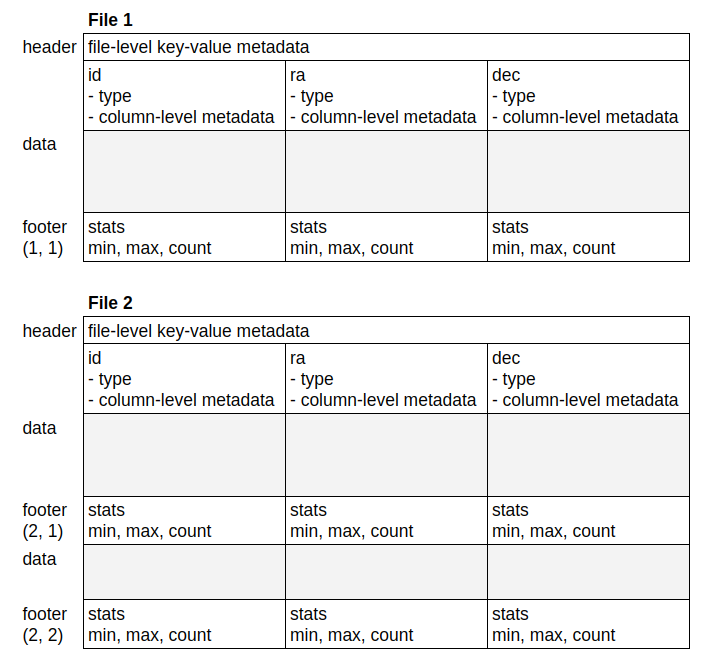
\includegraphics[width=0.9\textwidth]{leaf_files.png}
\caption{Example file layout of two parquet files of a dataset}
\label{fig:partitionedParquet}
\end{figure}

For very large datasets, it is helpful to have a single file that holds the common header information in all of the partitioned parquet files (assuming that they have homogeneous structure).
This \texttt{\_common\_metadata} file can be much smaller (and so faster to read) than a leaf parquet file.
The footers, however, will be different for every file, and some files may contain multiple footers if the data inside a single file is very large.
These footers can be concatenated into a single \texttt{\_metadata} file, and can provide valuable insight into the distribution of the data. 
A clever parquet reader can use this information to filter queries to only those partitions where certain values are possible.
See Figure~\ref{fig:parquetMetadata} for the layout of these parquet metadata files.

\begin{figure}
\centering
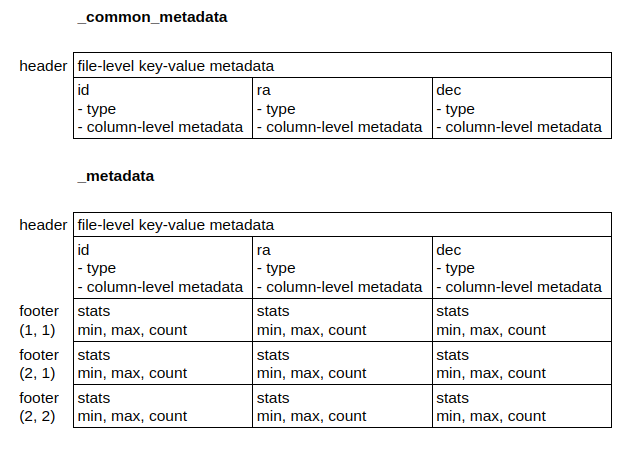
\includegraphics[width=0.9\textwidth]{metadata_files.png}
\caption{Example file layout of two supplemental parquet files of a dataset}
\label{fig:parquetMetadata}
\end{figure}

\subsubsection{collection.properties}\label{sec:collectionProperties}
A text file named \texttt{collection.properties} is REQUIRED for a catalog collection.
It marks the directory as containing a catalog collection, and so MUST be located in the 
root of the catalog collection.
It MUST be encoded in UTF-8, with one line per property, following the syntax \texttt{keyword = value}.
The ordering of the keywords is not important. 
The keywords MAY include many of those listed in Table~\ref{tab:properties}, with collection-specific fields shown in Table~\ref{tab:propertyRequirements}.

The text file may contain comment lines, beginning with the \texttt{'\#'} character.
An example \texttt{properties} file is shown in Listing~\ref{fig:exampleCollectionPropertiesFile}.

\begin{minipage}{\linewidth}
\begin{lstlisting}[caption=Example \texttt{collection.properties} file contents, label=fig:exampleCollectionPropertiesFile]
#HATS Collection
obs_collection=gaia_dr3
hats_primary_table_url=gaia
all_margins=gaia_5arcs gaia_1arcs
default_margin=gaia_5arcs
all_indexes=designation designation_index
\end{lstlisting}
\end{minipage}

\section{Performance Considerations}
Here, we will elaborate on several ways in which this format can be efficiently used. These insights come from our work with LSDB\footnote{\url{https://lsdb.io}}, a Python implementation of a package that works natively with HATS catalogs. \par

\subsection{Parquet Storage}\label{sec:parquetPerformance}
Firstly, we emphasize the need to use the Parquet column filtering. 
\textcolor{red}{KOSTYA NOTE - I don't understand the sentence about the standard practice and SQL/Python-like}
\textcolor{red}{MELISSA NOTE TO KOSTYA NOTE - I kind of agree, and don't know how to rephrase}
This is a standard practice in SQL-like workflows where users request only the necessary columns, but it is less common in Python-like workflows. 
Loading into memory only the columns that a user needs for scientific analysis, typically just a few out of the tens or hundreds available, significantly reduces the computational requirements for the analysis.  \par 

We can also split Parquet files into so-called row groups, splitting Parquet into chunks with a fixed number of rows. 
Parquet readers can skip over entire row groups if they don't contain relevant data, using the Parquet row group footer's min and max values for hints. 
This is especially effective when row groups are designed to match the access patterns of a specific scientific use case. 
For instance, if row groups are made to be small and they are sorted by the identification number of the survey, the retrieval of the individual rows by survey identification can be made much faster. 
This speed-up happens because we don't have to load the entire Parquet file into memory, but only the smaller row group, to retrieve the needed row with the required identification number.\par 
\textcolor{red}{KOSTYA NOTE - We never talk about how Parquet is good for block storage and network access}

\subsection{HTTP Services}
The fact that the data can be stored on the hard drive and served at rest to the users simplifies the cost structure for catalog providers. 
However, a user operating on the dataset, even if they are doing aggressive filtering and requesting a minimal number of rows at the end, will still have to transfer a large amount of data to their client, where the filtering is actually conducted. 
These limitations could become prohibitive if done over a network or with limited bandwidth. 
To alleviate that problem, it is possible to implement a server-side query in which the filtering operations are done server-side, and only the final dataset is sent to a user. 
Of course, this requires computational resources on the provider's side, but operates on a single file and will benefit from parquet storage optimizations from Section~\ref{sec:parquetPerformance}

\subsection{Cross-matching}
Finally, we want to highlight the exceptional performance possible when cross-matching HATS catalogs. 
Due to its spatial sharding, the cross-matching approach implemented in LSDB is competitive with the existing tools for small data, and is more efficient for large catalogs, starting with roughly one million rows. 
The key advantage lies in the fine-grained spatial partitioning: each data chunk is designed to fit comfortably into memory, allowing efficient parallel processing without memory bottlenecks. Users can increase the number of parallel computation units, and—provided the number of workers remains below the number of partitions and I/O throughput is sufficient—achieve near-linear scaling. \par 

For typical cases of large catalogs (billion+ rows), cross-matching on a single core is around 5 to 15\% slower than the pure I/O speed. 
As discussed above, selecting only specific columns and parallelizing the work can drastically improve performance.   

\section{Role within the VO Architecture}

\begin{figure}
\centering

\includegraphics[width=0.9\textwidth]{role_diagram.pdf}
\caption{Architecture diagram for this document}
\label{fig:archdiag}
\end{figure}

Figure~\ref{fig:archdiag} shows the role this document plays within the IVOA architecture.

HATS is designed to be compatible with existing VO spatial indexing frameworks, such as HEALPix \citep{gorski:healpix} and MOC (Multi-Order Coverage maps) \citep{ivoa:MOC}. \par
It builds upon the nested HEALPix tessellation scheme, which provides a hierarchical and uniform way to partition the celestial sphere. This structure is central to HATS: both the storage layout and the spatial indexing are defined in terms of HEALPix pixels.
The full footprint of the catalog can alternatively be represented by a MOC, as it is a list of HEALPix pixels, at many different HEALPix orders. \par 

The HATS format can be made to be compatible with the TAP query by implementing a translation layer between the TAP query language. 
We have explored some initial implementation of such functionality, but the implementation details will always depend on the language used to handle the Parquet files. \par

We are closely following the development of the VOParquet format and aim to implement it as a part of HATS catalogs.

\appendix
\section{Changes from Previous Versions}
No previous versions yet.

% \bibliography{ivoatex/ivoabib,ivoatex/docrepo}
\begin{thebibliography}{}

\harvarditem{Bradner}{1997}{std:RFC2119}
Bradner, S.  \harvardyearleft 1997\harvardyearright , `Key words for use in
  {RFCs} to indicate requirement levels', RFC 2119.
\newblock \url{http://www.ietf.org/rfc/rfc2119.txt}.

\harvarditem{Masci et al.}{2019}{ztf:Masci2019}
Masci, F.~J., et al. \harvardyearleft 2019\harvardyearright,
`The Zwicky Transient Facility: Data Processing, Products, and Archive',
PASP, 131, 018003. \url{https://ui.adsabs.harvard.edu/abs/2019PASP..131a8003M}.

\harvarditem{Bellm et al.}{2019}{ztf:Bellm2019}
Bellm, E.~C., et al. \harvardyearleft 2019\harvardyearright,
`The Zwicky Transient Facility: System Overview, Performance, and First Results',
PASP, 131, 018002. \url{https://ui.adsabs.harvard.edu/abs/2019PASP..131a8002B}.

\harvarditem{Fernique et al.}{2019}{ivoa:MOC}
Fernique, P., Boch, T., Donaldson, T., Durand, D., O'Mullane, W., Reinecke, M., \& Taylor, M.  
\harvardyearleft 2019\harvardyearright,  
*MOC - HEALPix Multi-Order Coverage map Version 1.1*,  
IVOA Recommendation 07 October 2019.  
\url{https://ui.adsabs.harvard.edu/abs/2019ivoa.spec.1007F}.

\harvarditem{G{\'o}rski et al.}{2005}{gorski:healpix}
G{\'o}rski, K.~M., Hivon, E., Banday, A.~J., Wandelt, B.~D., Hansen, F.~K., Reinecke, M., \& Bartelmann, M.  
\harvardyearleft 2005\harvardyearright,  
`HEALPix: A Framework for High-Resolution Discretization and Fast Analysis of Data Distributed on the Sphere',  
*Astrophysical Journal*, **622**, 759–771.  
\url{https://ui.adsabs.harvard.edu/abs/2005ApJ...622..759G}.

\end{thebibliography}
\end{document}

